\pagenumbering{arabic} % numbering: 1,2,3,...
    \section*{CHƯƠNG 1. GIỚI THIỆU CHUNG} 
        \addcontentsline{toc}{section}{\numberline{}CHƯƠNG 1. GIỚI THIỆU CHUNG} % Reference to content

\setcounter{section}{1} 
    \setcounter{subsection}{0}
        \setcounter{figure}{0}
            \setcounter{table}{0}
%%--------------------------------------------------------

\subsection{Vai trò của thiết bị đọc ghi màn hình cột bơm xăng dầu}

\hspace{1cm} Công nghệ số mang đến ngày càng nhiều lợi ích to lớn về mặt tiện dụng, hiệu quả và tiết kiệm thời gian cho doanh nghiệp cũng như người dùng. Từ đó, nhu cầu lớn về chuyển đổi số được phát sinh. Các thông tin giao dịch, hóa đơn trên giấy tờ ngày càng được thay thế bằng các giao dịch, hóa đơn điện tử, thuận tiện cho truyền tải thông tin, lưu trữ và quản lý. Các hệ thống trạm xăng và cột bơm cũng không phải ngoại lệ với nhu cầu đó, các giao dịch, lượt bơm xăng cũng cần được ghi lại dưới dạng dữ liệu số để gửi lên máy chủ của doanh nghiệp, thuận tiện lưu trữ và thống kê một cách chính xác, ổn định và giảm hoặc triệt tiêu những lỗi con người có thể gây ra.

Những cột bơm mới được bán gần đây cũng đã được sản xuất tích hợp chức năng xuất hóa đơn điện tử. Nhưng còn một lượng rất lớn những cây xăng với công nghệ cũ vẫn còn đạt tiêu chuẩn và sử dụng tốt được ở nhiều trạm bơm trên khắp cả nước, việc bỏ hẳn những cây xăng này đi thay bằng những cây xăng công nghệ mới sẽ tốn nhiều thời gian và chi phí đầu tư, gây lãng phí cũng như thải nhiều rác thải điện tử hơn cho môi trường. Từ đó xuất hiện nhu cầu cải tiến những cây xăng cũ để xuất được hóa đơn điện tử, chi phí và thời gian doanh nghiệp bỏ ra sẽ được tối ưu hơn.

Từ yêu cầu trực tiếp của doanh nghiệp, báo cáo này được viết để đưa ra phương án thiết kế và triển khai hệ thống có thể đọc ghi và giải mã, phân tích dữ liệu màn hình cây xăng, từ đó phát hiện được các lần giao dịch và lưu trữ, quản lý các lượt giao dịch - lượt bơm xăng đó.


\subsection{Khái quát về yêu cầu và chức năng của hệ thống}



\begin{figure}[!ht]
    \centering
    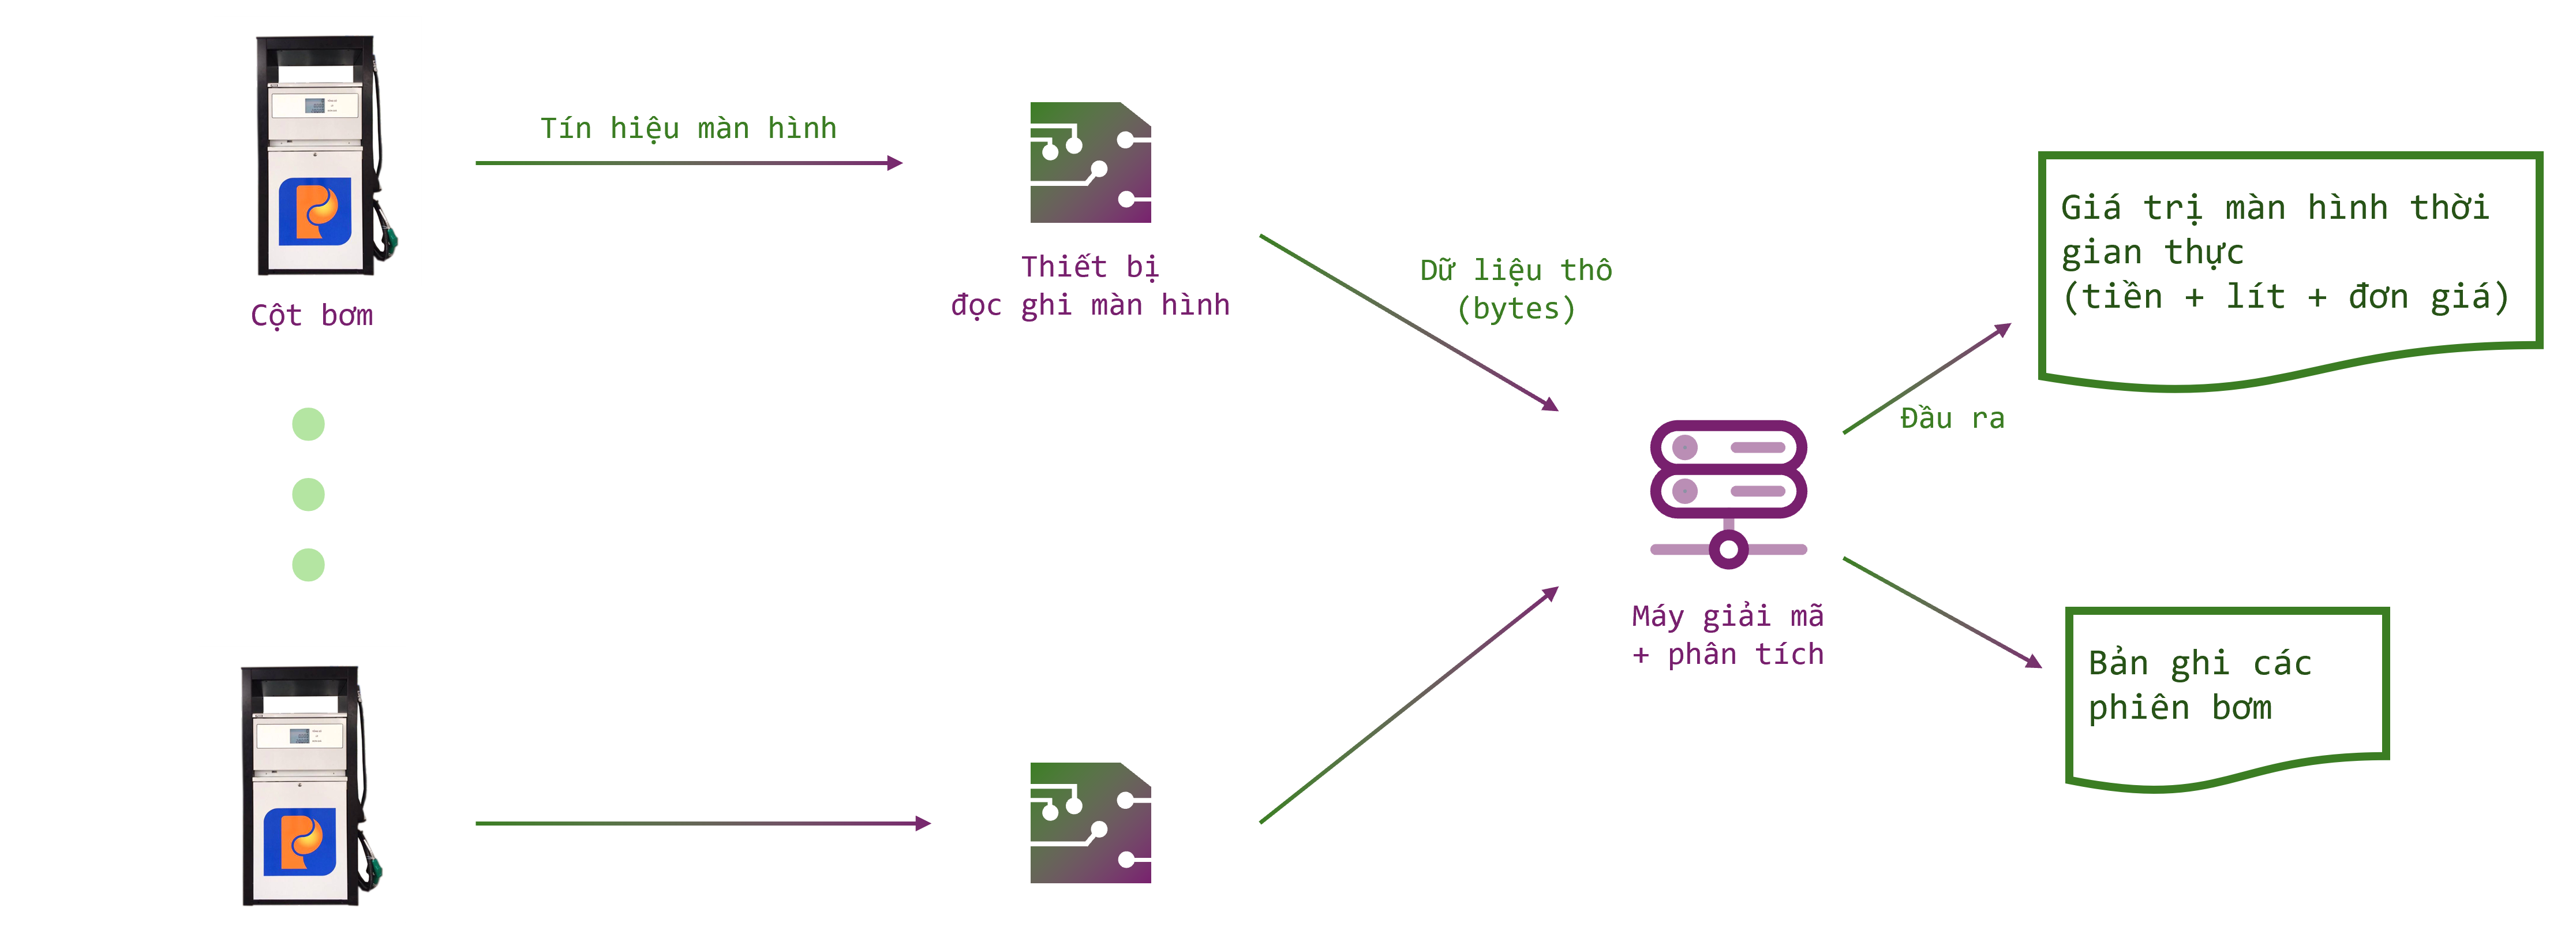
\includegraphics[width=1.0\linewidth]{Figures/Chap1_proj-purpose.png}
    \caption{Minh họa mục tiêu đầu ra của hệ thống}
    \label{fig:hinh1.1}
\end{figure}

Mục tiêu là thiết kế thiết bị đọc ghi và giải mã màn hình cây xăng đáp ứng những nhu cầu sau:

 \textbf{1. \quad Giám sát số liệu hiển thị trên cột bơm theo thời gian thực}

 Hệ thống có thể đọc và hiển thị trực tiếp dữ liệu cột bơm theo thời gian thực bao gồm: số tiền, số lít và đơn giá. Người dùng có thể theo dõi trạng thái hiển thị của cột bơm ngay tại phòng điều khiển mà không cần quan sát trực tiếp màn hình cột.
 

 \textbf{
    2. \quad  Phát hiện các lượt bơm hoàn chỉnh
 }

 Thông qua các số liệu thời gian thực (số tiền, số lít, đơn giá) của cột bơm, hệ thống phát hiện được đâu là bắt đầu và kết thúc của một lượt bơm xăng, thông báo một lượt bơm/hóa đơn hoàn chỉnh.


 \textbf{
    3. \quad Lưu trữ và hiển thị các lượt bơm
 }

 Các lượt bơm được lưu trữ trong cơ sở dữ liệu, tạo cơ sở để có thể xuất các hóa đơn điện tử.


 \textbf{
    4. \quad Hỗ trợ điều khiển từ xa
 }

 Việc ghi dữ liệu cột bơm có thể được điều khiển bật tắt từ xa, thông qua giao diện phần mềm.


 \textbf{
    5. \quad Cập nhật phần mềm từ xa (OTA)
 }

 Hỗ trợ cập nhật phần mềm từ xa, cho phép người dùng cập nhật phiên bản mới từ giao diện người dùng để có tối ưu những tính năng, tiện ích mới nhất từ phiên bản phần cứng đã có.

Thông qua việc triển khai mục tiêu trên, đề tài hướng tới tạo ra một hệ thống đọc và giải mã màn hình cây xăng hoàn chỉnh, đáp ứng nhu cầu quan sát từ xa các cột bơm theo thời gian thực, tự động phát hiện và ghi lại được các lượt bơm, tạo tiền đề để phát triển các ứng dụng như là xuất hóa đơn điện tử, thanh toán không chạm, và các ứng dụng khác.

\subsection{Phạm vi nghiên cứu}

\hspace{1cm} Thiết bị đọc ghi màn hình cột bơm xăng dầu có thể đọc ghi và giải mã loại cột bơm truyền thống có đặc điểm sau:
\begin{itemize}
   \item Hãng sản xuất: ZCheng
   \item Loại cáp màn hình: 8P 3.96mm
   \item Số lượng chân cáp: 8
   \item Số chân tín hiệu của cáp: 3
   \item Giao thức: SPI
   \item Độ lớn frame: 22 byte
   \item Bit rate: 400Kb/s
   \item Tần số frame: 100Hz
\end{itemize}
Đây là loại cột bơm cũ phổ biến tại các trạm xăng trên thị trường. Phạm vi chức năng của hệ thống bao gồm:

 \textbf{1. \quad Giám sát số liệu hiển thị trên cột bơm theo thời gian thực}

 Thu và giải mã dữ liệu SPI gửi tới màn hình thiết bị. Hiển thị giá trị màn hình (số tiền, số lít, đơn giá) theo thời gian thực trên giao diện người dùng.

  \textbf{
    2. \quad  Phát hiện các phiên bơm hoàn chỉnh
 }

 Sau khi bơm xăng, người vận hành dừng bơm một thời gian (5s) hoặc nhấn nút reset để bắt đầu phiên bơm mới, thiết bị phát hiện và ghi lại giá trị màn hình hiện tại thành một phiên bơm.

  \textbf{
    3. \quad Lưu trữ và hiển thị các lượt bơm
 }

 Các bản ghi phiên bơm được lưu vào cơ sở dữ liệu ngay trên máy tính nội bộ và hiển thị lên giao diện quản lý

 \textbf{
    4. \quad Hỗ trợ điều khiển từ xa
 }

Thiết bị đọc màn hình cây xăng có 2 relay đóng ngắt có thể nối nối tiếp vào cột bơm. Từ giao diện quản lý, có thể điều khiển relay đóng ngắt bằng nút ấn trên giao diện.


 \textbf{
    5. \quad Cập nhật phần mềm từ xa (OTA)
 }

 Từ giao diện quản lí, có thể tải (upload) file phần mềm dạng mã nhị phân, gửi cho thiết bị đọc màn hình để thiết bị tự cập nhật. 

\subsection{Phương pháp nghiên cứu}

\hspace{1cm} Bối cảnh màn hình cây xăng là các màn hình cũ, không có tài liệu cụ thể về thiết phần cứng và giao thức.

\begin{figure}[!ht]
    \centering
    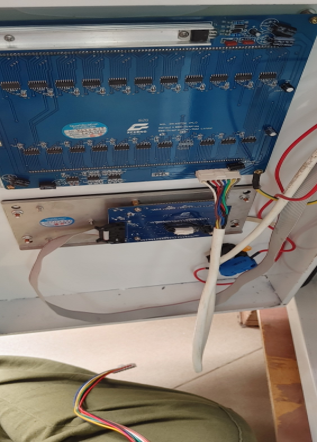
\includegraphics[width=0.5\linewidth]{Figures/Chap1_Zcheng-screen-hardware.png}
    \caption{Mạch phần cứng màn hình cây xăng hãng ZCheng}
    \label{fig:hinh1.1}
\end{figure}

Do đó, cần khảo sát tín hiệu màn hình. Sử dụng mạch thu và phần mềm của Logic Analyzer để thu tín hiệu theo các bước sau:

- Sử dụng đồng hồ đo áp, xác định các chân nguồn, đất, tín hiệu và các chân có điện áp cao (để tránh cắm chân Logic Analyzer vào các chân có điện áp cao này).

- Sử dụng mạch cứng và phần mềm Logic Analyzer nối vào các chân tín hiệu tới màn hình để thu các tín hiệu. Đồng thời, sử dụng máy quay quay lại màn hình hiển thị trong quá trình thu.

- Thực hiện các thao tác phổ biến: reset màn hình, bơm xăng, preset màn hình (đặt trước giá trị tiền hoặc lít cần bơm) rồi ghi lại tín hiệu và video màn hình trong quá trình vận hành thao tác.

- Khảo sát tín hiệu, so sánh tín hiệu với giá trị hiển thị trên màn hình để xác định:

\begin{itemize}
   \item Vị trí các chân (nguồn, đất, cấp xung, dữ liệu, ...)
   \item Giao thức sử dụng (SPI), dấu hiệu bắt đầu và kết thúc một gói tin
   \item Ý nghĩa các byte trong gói tin
\end{itemize}

Từ đó, chế tạo mạch thu gói tin theo giao thức SPI và thiết kế phần mềm giải mã.

\subsection{Cấu trúc đồ án}

Nội dung được trình bày ở các chương tiếp theo bao gồm: 
\begin{itemize}
   \item Tổng quan lý thuyết và công nghệ: Trình bày các nền tảng lý thuyết và mô tả các công nghệ được sử dụng trong thiết kế.
   \item Thiết kế hệ thống sản phẩm: Bao gồm sơ đồ các khối chức năng của thiết bị đọc ghi màn hình và phần mềm giải mã, cùng với thiết kế chi tiết (mạch cứng và phần mềm) từng khối, trình tự giao tiếp giữa các khối.
   \item Triển khai và thử nghiệm: Thử nghiệm thiết bị trên màn hình cột bơm tại hiện trường, đánh giá kết quả.
   \item Kết luận và hướng phát triển.
\end{itemize}

\subsection{Kết luận chương}

\hspace{1cm} Trong chương này, em đã đưa ra bối cảnh thực tế của bài toán, giải thích nhu cầu thực tế của thiết bị đọc ghi màn hình cây xăng, cùng với lợi ích mà nó mang lại trong quá trình phát triển và chuyển đổi số.

Đồng thời, chương này liệt kê các yêu cầu kĩ thuật cụ thể, cách tiếp cận bài toán từ đó đưa ra hướng thiết kế và triển khai tiếp theo.

